%===================================================================================
\subsection{CU27 Ver diagrama de gantt}
{
\justify
\color{blue}{\textbf{Objetivo}}
}

%------------------------------------------------------------------
\justify
Permite al Lider de proyecto visualizar el diagrama de gantt con las tareas del proyecto.
%------------------------------------------------------------------
{
\justify
\color{blue}{\textbf{Diseño}}
}
%-------------------------------------------------------------------------------
\justify
En la figura \ref{fig:IU27} se muestra la pantalla, en donde permité al Lider de proyecto visualizar el diagrama de gantt con las tareas del proyecto.

\begin{figure}[htb]
\centering
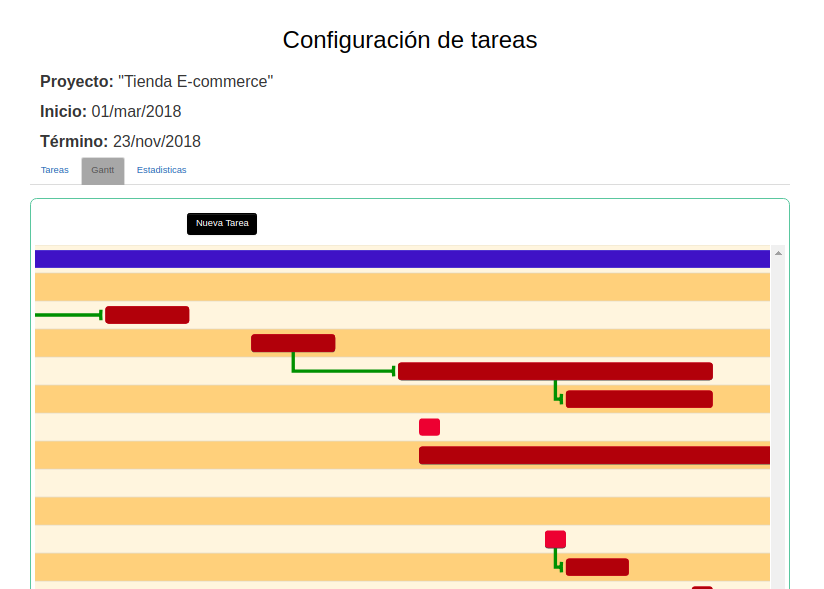
\includegraphics[width=0.8\textwidth]{./images/cu27-ver-diagrama-gantt.png}
\caption{Ver diagrama de gantt.} \label{fig:IU27}
\end{figure}